\section{XOR}


Anteriormente, habíamos logrado separar clases de ejemplares siempre y cuando estos se pudieran modelar en un plano linealmente separable. Hasta ahora había sido un reto importante (no logrado) hacer clasificaciones de ejemplares distribuidos en un plano no separable linealmente, como lo es \emph{la función XOR} donde, tenemos que las respuestas positivas se encuentran en una diagonal opuesta a las respuestas negativas y no hay manera de separar a los blancos de los negros con una sola frontera lineal, lo que hace imposible separar con un solo perceptrón. Entonces notamos que necesitamos de dos líneas que nos permitan separar el plano. Así llegamos a la idea que necesitamos más de una capa, que nos permita hacer la siguiente separación del plano.

\begin{figure}[H]
 \centering
 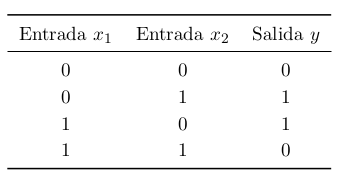
\includegraphics[scale=0.5]{../Figuras/TablaXor.png}
 \caption{Tabla de verdad para la función XOR.}
 \label{fig:tablaXOR}
\end{figure}

\begin{figure}[H]
 \centering
 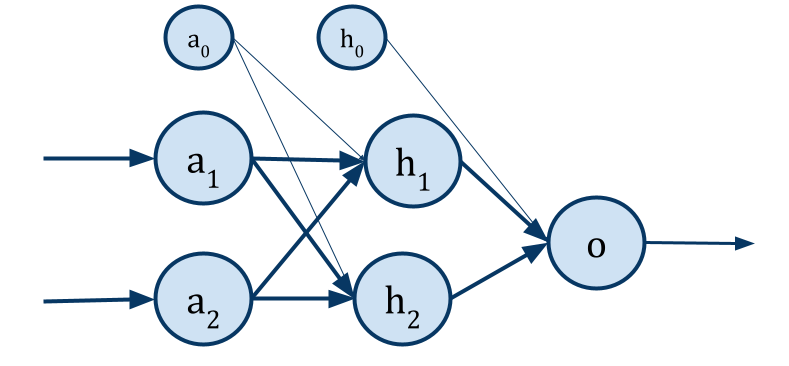
\includegraphics[scale=0.3]{../Figuras/XOr.png}
 \caption{Perceptrón para la función XOR, con una capa oculta.}
 \label{fig:pXor}
\end{figure}



En la tabla de verdad notamos que para la función XOR, cuando la suma de las entradas es:
\begin{itemize}
 \item par (tomando en cuanta al cero como par) la salida es $0$.
 \item impar la salida es $1$.
\end{itemize}


Para poder aprender la función únicamente tenemos que añadir una capa intermedia, la llamada capa oculta. Esta capa será la responsable de tomar las características de los vectores de entrada.


Ahora para la función tenemos dos entradas, una capa oculta (con dos neuronas) y una salida. Las neuronas en la capa oculta nos permitirán dividir el plano. Así, una solución sería que las neuronas ocultas denotadas por $h$ (\emph{hidden} de oculto en inglés) compartan pesos, la primera neurona $h_1$ haría la función $OR$, haciendo la distinción entre las entradas $0 0$, la segunda neurona $h_2$ haría la función $NAND$ haciendo posible distinguir el vector de entrada $1 1$, una vez obtenido estos resultados de la capa oculta la neurona de salida $o$ de output se encargara de distinguir la intersección entra estas, ejecutando la función $AND$. En resumen, la función \emph{XOR} la podemos rescribir como:


\begin{equation}
 \begin{split}
    XOR &= (x_{1} \vee x_{2}) \wedge \neg(x_{1} \wedge x_{2}) \\
    XOR &= AND (OR(x_{1}, x_{2}), NAND(x_{1}, x_{2}))
 \end{split}
\end{equation}

\begin{figure}[H]
 \centering
 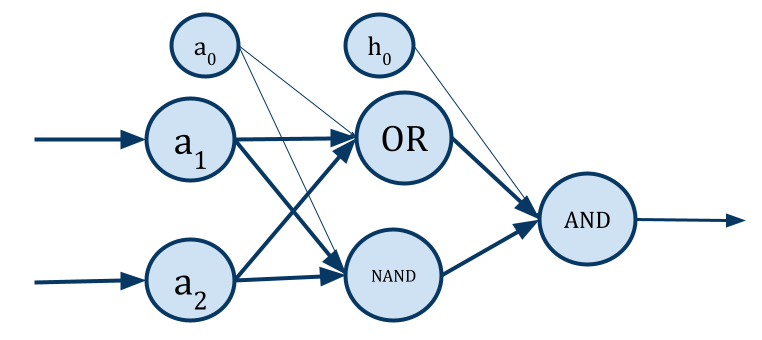
\includegraphics[scale=0.3]{../Figuras/xor.png}
 \caption{Solución para perceptrón de la función XOR.}
 \label{fig:pXorSol}
\end{figure}





